\begin{frame}{Formal Setting}
  \begin{itemize}
    \item measure space, probability measure, random vector, subvector, complementary vector, pdf
    \item measure space of square integrable functions
    \item inner product
    \item norm
  \end{itemize}
  
\end{frame}

\begin{frame}{Decompose model into interpretable components} % What is it?
\begin{block}{General Form}
\[
  \begin{aligned}
    y(\boldsymbol{X}) 
    &= \sum_{u \subseteq \{1,\dots,N\}} y_{u}(\boldsymbol{X}_u) \\[3pt]
    &= y_{\emptyset} 
       + \big( y_{\{1\}}(\boldsymbol{X}_1) + \dots + y_{\{N\}}(\boldsymbol{X}_N) \big) \\[2pt]
    &\quad + \big( y_{\{1, 2\}}(\boldsymbol{X}_1,\boldsymbol{X}_2) 
                 + y_{\{1, 3\}}(\boldsymbol{X}_1,\boldsymbol{X}_3) + \dots \big) \\[2pt]
    &\quad + \big( y_{\{1, 2, 3\}}(\boldsymbol{X}_1,\boldsymbol{X}_2,\boldsymbol{X}_3) + \dots \big) 
       + \dots + y_{\{1, \dots, N\}}(\boldsymbol{X}_1, \dots, \boldsymbol{X}_N)
  \end{aligned}
\]
\end{block}

  \begin{itemize}
    \item $y$ : Model
    \item $y_u$ : Component functions for subset $u$
    \item Assumption: $X_1, \dots, X_N$ are independent
  \end{itemize}
\end{frame}

\begin{frame}{Ensure Uniqueness and Interpretability of the Components} % What conditions do we need?
  \begin{block}{Strong Annihilating Conditions}
    \[
      \int_{\mathbb{R}} y_u(\boldsymbol{x}_u) f_{\{i\}}(x_i) \, d\nu(x_i) = 0 \quad \text{for} \ i \in u \neq \emptyset.
    \]
  \end{block}
  \begin{itemize}
    \item Ensures unique component functions
    \item Applies under independent (product-type) input distributions
  \end{itemize}
    \[
    \mathbb{E}[y_u(\boldsymbol{X}_u)] = 0
  \]
  \[
    \mathbb{E}[y_u(\boldsymbol{X}_u) y_v(\boldsymbol{X}_v)] = 0 \quad (u \neq v)
  \]
\end{frame}


\begin{frame}{Recursive Form of the Components} % How do we construct it?
    \[
    y_{\emptyset} = \int_{\mathbb{R}^N} y(\boldsymbol{x}) \prod_{i=1}^{N} f_{\{i\}}(x_i) \, d\nu (x_i) = \mathbb{E}[y(\boldsymbol{X})].
    \]
\begin{equation}
    y_u(\boldsymbol{X}_u) 
    = \int_{\mathbb{R}^{N- |u|}} 
        y(\boldsymbol{X}_u, \boldsymbol{x}_{-u}) 
        \prod_{i=1, i \notin u}^{N} f_{\{i\}}(x_i) 
        \, d\nu (x_i) 
      - \sum_{v \subsetneq u} y_v(\boldsymbol{X}_v).
    \label{eq:fanova_components_classical}
\end{equation}
  \begin{itemize}
    \item $f_{-u}$ : marginal density of variables not in $u$
    \item Components solved sequentially by increasing order
  \end{itemize}
\end{frame}

\begin{frame}{Recursive Form Example}
  \begin{itemize}
    \item $N = 3$
  \end{itemize}
    \[
    y_{\emptyset} = \int_{\mathbb{R}^3} y(\boldsymbol{x}) \prod_{i=1}^{3} f_{\{i\}}(x_i) \, d\nu (x_i) = \mathbb{E}[y(\boldsymbol{X})].
    \]
  \begin{itemize}
    \item $u = \{1\}$ $\rightarrow$ $v = \emptyset$
  \end{itemize}
    \begin{equation*}
    y_{\{1\}}(X_1) 
    = \int_{\mathbb{R}^{2}} 
        y(X_{1}, x_{2}, x_{3}) 
        \prod_{i=2}^{3} f_{\{i\}}(x_i) 
        \, d\nu (x_i) 
      -  y_{\emptyset} = \mathbb{E}[y(X_1, X_2, X_3)|X_1 = x_1] - y_{\emptyset}.
\end{equation*}
  \begin{itemize}
    \item $u = \{1,2\}$ $\rightarrow$ $v = \{1\}, \{2\}, \emptyset$
  \end{itemize}
    \begin{align*}
    y_{\{1,2\}}(X_1, X_2) 
    &= \int_{\mathbb{R}} 
        y(X_1, X_2, x_3) 
        f_{\{3\}}(x_3) 
        \, d\nu (x_3) 
      -  y_{\{1\}}(X_1) -  y_{\{2\}}(X_2) - y_{\emptyset} \\
    &= \mathbb{E}[y(X_1, X_2, X_3)|X_1 = x_1, X_2 = x_2] - y_{\{1\}}(X_1) - y_{\{2\}}(X_2) - y_{\emptyset}.
\end{align*}
  
\end{frame}


\begin{frame}{Example: Independent MVN} % Example of a 2D function
  \begin{align*}
    y(x_1, x_2) = 2x_1 + x_2^{2} + x_1 x_2
  \end{align*}
\[
(X_1, X_2)^\mathsf{T} \sim \mathcal{N}\!\left(
\begin{pmatrix}0 \\ 0\end{pmatrix},
\begin{pmatrix}
1 & \rho \\ 
\rho & 1
\end{pmatrix}
\right),
\]
\[
X_1 \mid X_2=x_2 \sim \mathcal{N}(\rho x_2, 1-\rho^2), \quad
X_2 \mid X_1=x_1 \sim \mathcal{N}(\rho x_1, 1-\rho^2).
\]
Components:
\begin{equation*}
    y_{\emptyset} = 0, \qquad
    y_{\{1\}}(x_1) = 2x_1, \qquad
    y_{\{2\}}(x_2) = x_2^{2}, \qquad
    y_{\{1,2\}}(x_1, x_2) = x_1 x_2.
\end{equation*}
\end{frame}


\begin{frame}{Example: 2D Function} % How does it look?
  \begin{columns}
    \column{0.5\textwidth}
      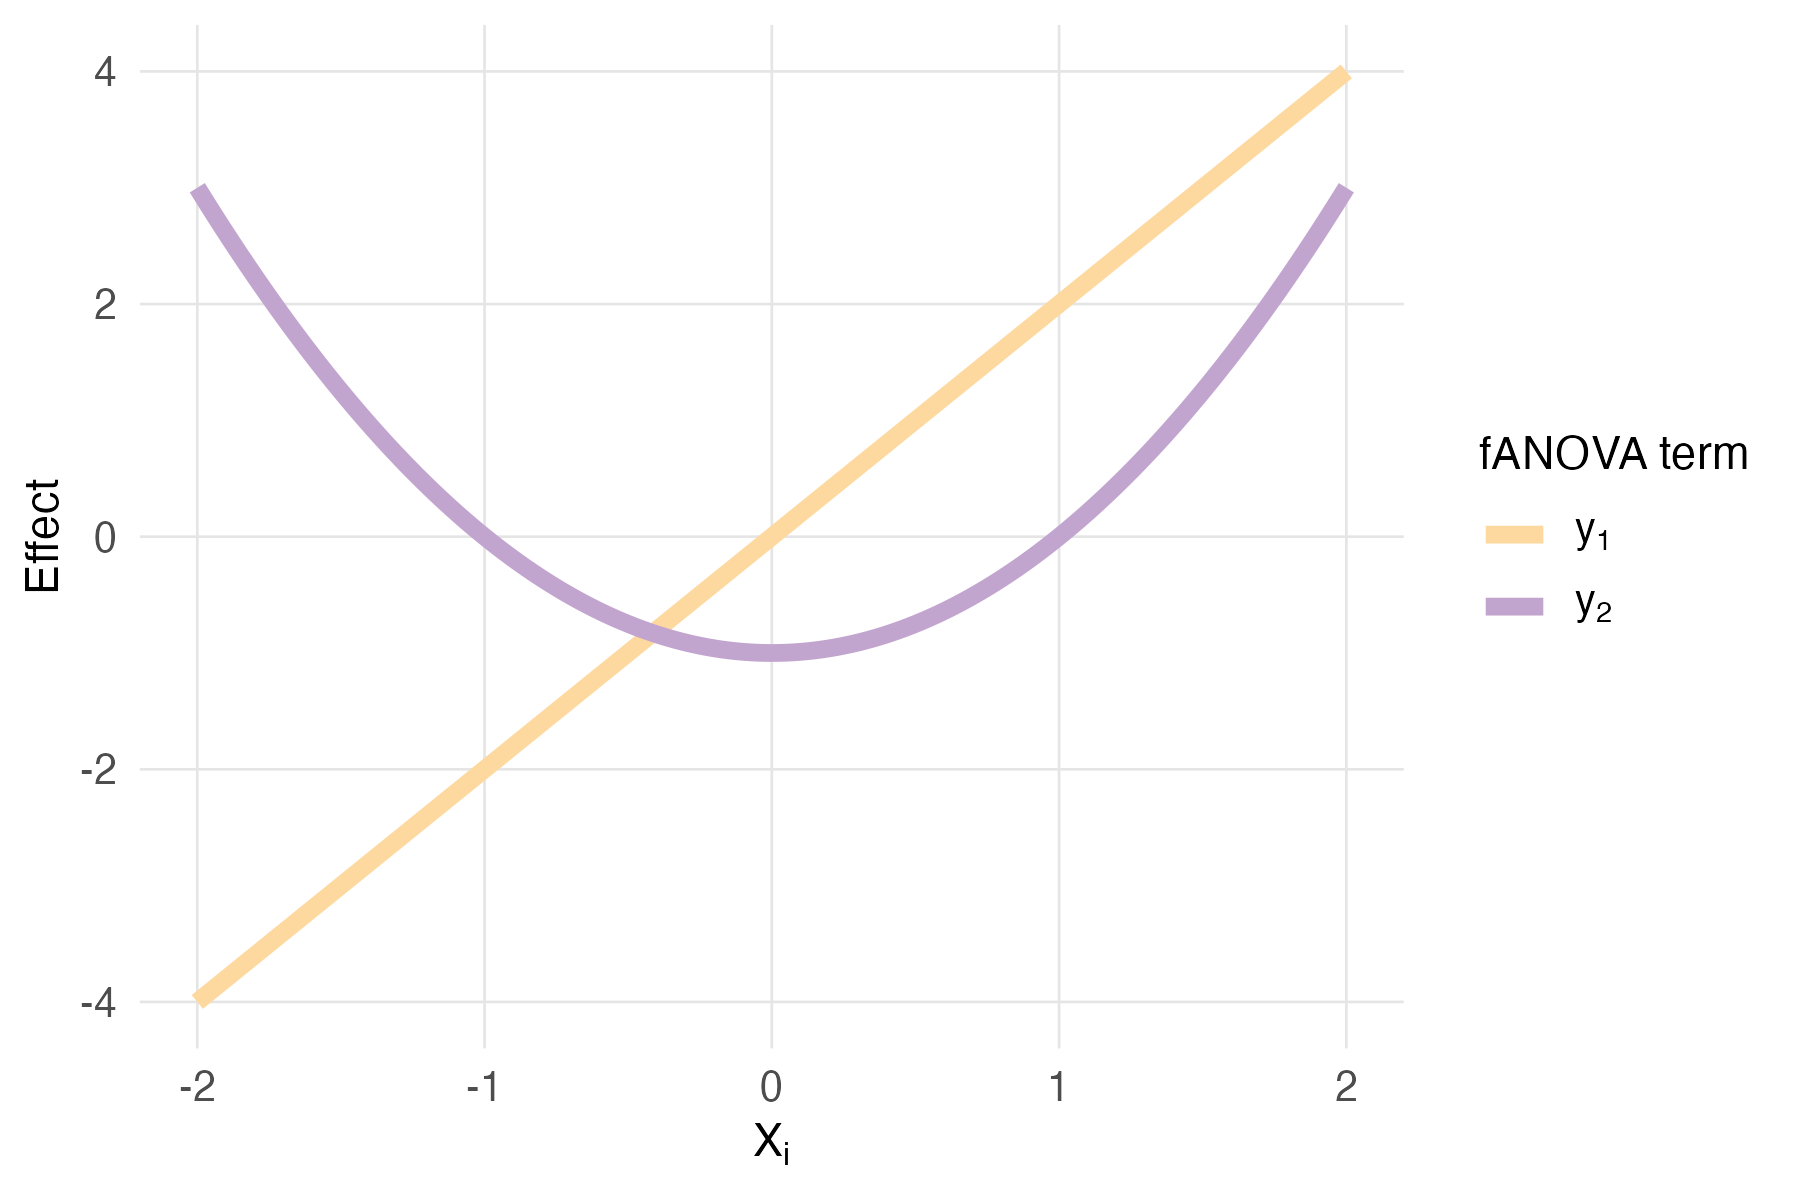
\includegraphics[width=\linewidth]{../images/experiment_section/classical_ex_1_a1p20_a2p00_a11p00_a22p10_a12p10_rhop00_main.png}
    \column{0.5\textwidth}
      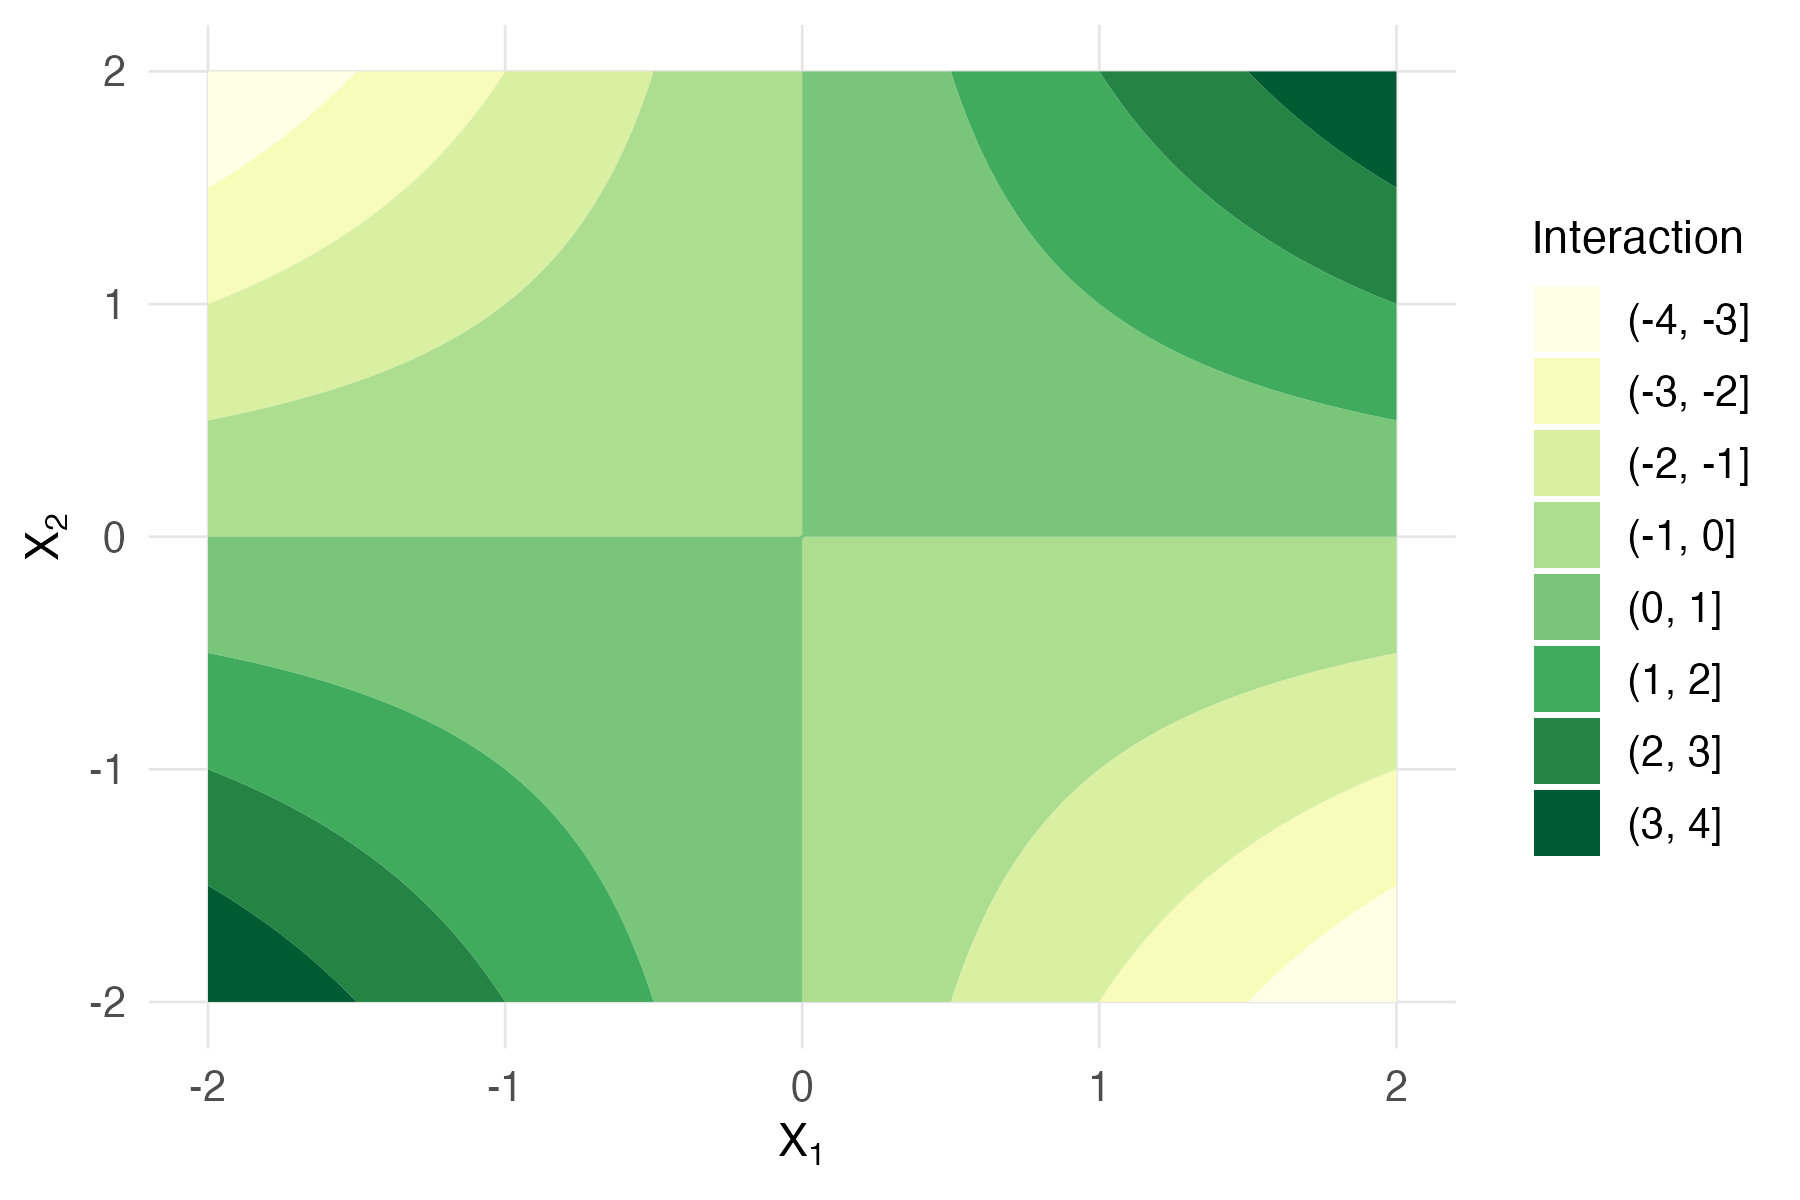
\includegraphics[width=\linewidth]{../images/experiment_section/classical_ex_1_a1p20_a2p00_a11p00_a22p10_a12p10_rhop00_interaction.png}
  \end{columns}
\end{frame}

% fANOVA through lens of Orthogonal Projections
\begin{frame}{Reminder: Definition of Orthogonal Projection} % How do we define it?
  \begin{align}
    \Pi_{\mathcal{G}}y = \arg\min_{g \in \mathcal{G}} \|y - g\|^2
= \arg\min_{g \in \mathcal{G}} \mathbb{E}[(y(\boldsymbol{X}) - g(\boldsymbol{X}))^2].
\end{align}
  \begin{itemize}
    \item $\mathcal{G}$ : linear subspace of $\mathcal{L}^2$ we project onto
    \item $g$ all functions in the subspace
  \end{itemize}
\end{frame}

\begin{frame}{fANOVA as Orthogonal Projection} % How does it relate to orthogonal projection?
  \begin{align*}
    \Pi_{\mathcal{G}_0}y
    &= \arg \min_{g_0 \in \mathcal{G}_0} \|y - g_0\|^2 \\ 
    &= \arg \min_{a \in \mathbb{R}} \mathbb{E}[(y(\boldsymbol{X}) - a)^2] \\ 
    &= \mathbb{E}[y(\boldsymbol{X})] = y_{\emptyset}.
\end{align*}
  \begin{align*}
    (\Pi_{\mathcal{G}_u}y)(.) - \sum_{v \subsetneq u} y_v(.)
    &= \arg \min_{g_u \in \mathcal{G}_u} \|y - g_u\|^2 - \sum_{v \subsetneq u} y_v(.)\\
    &= \arg \min_{g_u \in \mathcal{G}_{u}} \mathbb{E}[(y(\boldsymbol{X}) - g_u(.))^2] - \sum_{v \subsetneq u} y_v(.)\\
    &= \mathbb{E}[y(\boldsymbol{X}) \mid X_{u} = .] - \sum_{v \subsetneq u} y_v(x) = y_u(.).
\end{align*}
  
\end{frame}


\begin{frame}{Equality to Hoeffding Decomposition} % How does it relate to Hoeffding?
  \begin{block}{Hoeffding Decomposition}
    \begin{align}
    y(\boldsymbol{X})
=
\sum_{A \subseteq D} 
y_A(\boldsymbol{X}_A),
\qquad
D := \{1,\dots,N\},
\end{align}
where, for each $A \subseteq D$, the component function $y_A$ is defined by:
\begin{align}\label{eq:hoeffding_components}
    y_A(\boldsymbol{X}_A)
=
\sum_{B \subseteq A}
(-1)^{|A|-|B|}
\,\mathbb{E}\!\left[
  y(\boldsymbol{X}) 
  \,\middle|\, 
  \boldsymbol{X}_B
\right],
\end{align}
  where $y_u$ are orthogonal components.
  \end{block}
  \begin{itemize}
    \item Classical fANOVA and Hoeffding decomposition yield same components under zero-centered inputs
    \item Both assume independence of input variables
  \end{itemize}
  
\end{frame}


